\documentclass[a4paper, 12pt]{report}
\usepackage[utf8]{inputenc}
\usepackage{graphicx}
\usepackage{xcolor}
\usepackage{appendix}
\usepackage{hyperref}
\usepackage[top=2cm, bottom=2cm, left=2cm, right=2cm]{geometry}
\usepackage[francais]{babel}
\usepackage{hyperref}
\hypersetup{
    colorlinks=true,
    linkcolor=black,
    urlcolor=black,
    linktoc=all
}

\usepackage{fancyhdr}
\usepackage{lastpage}

\addtocontents{toc}{\protect\thispagestyle{fancy}}

\pagestyle{fancy}
\setlength\headheight{12mm}
\fancyhf{}
\lhead{
\includegraphics[height=1cm]{../../public/images/Logo-spf-sm.png}}
\chead{}
\rhead{
\includegraphics[height=8mm]{../../public/images/Logo-entremploi-sm.png}}
\lfoot{\today}
\cfoot{}
\rfoot{page \thepage \ / \pageref{LastPage}}

\title{Entr'Emploi}
\author{MAILLARD Noé MILSONNEAU Jean}

\begin{document}

\begin{titlepage}
	\thispagestyle{empty}
    \centering
    {\bfseries\Large
    		Site internet EntrEmploi\\
        \today\\
        \vskip3cm
        
\includegraphics{../../public/images/Logo-entremploi-md.png}
        \vskip15mm
        
\includegraphics{../../public/images/Logo-spf.png}
        \vskip3cm
        Maillard Noé, Milsonneau Jean\\
    }
    \normalsize
\end{titlepage}

\tableofcontents

\chapter{Présentation du site}
\section{Page d’accueil}

\includegraphics[width=16cm]{homePage.png}
\\
La page d'accueil contient des articles de présentation de l'action d'Entr'Emploi et un carrousel d'images, le tout est modifiable par la personne en charge du contenu du site.
\section{Prestations}
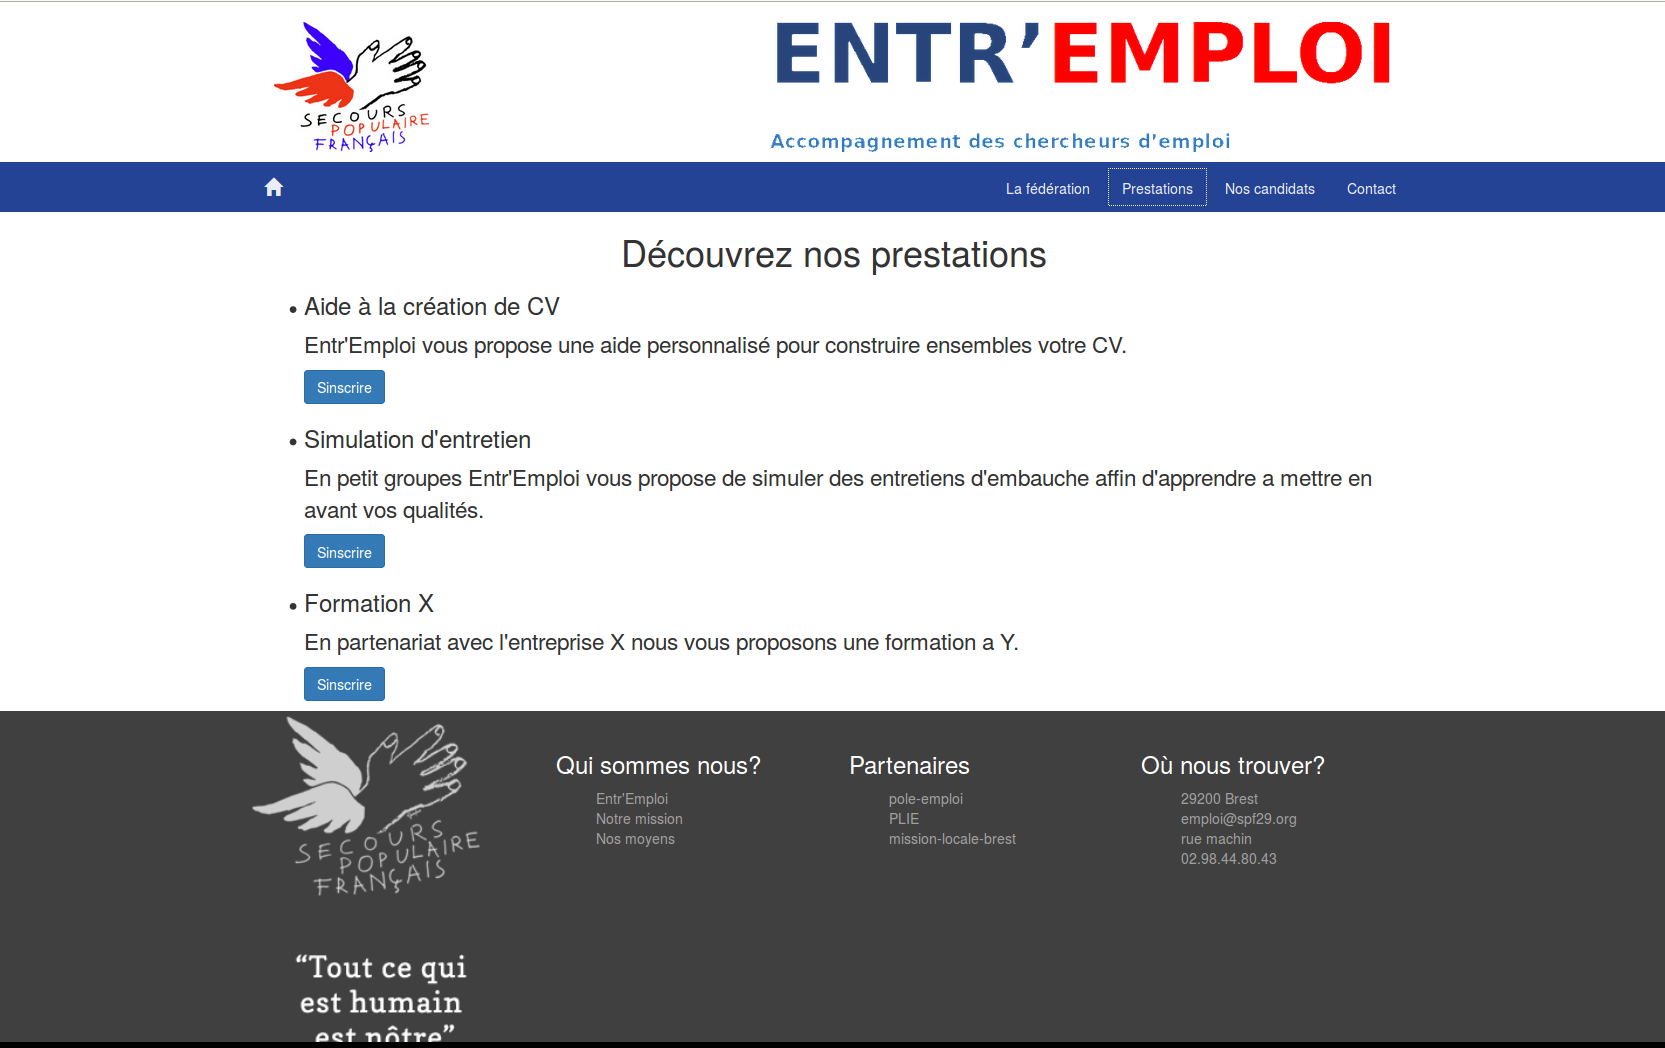
\includegraphics[width=16cm]{prestations.png}
\\
La page prestations offre un liste de prestations proposé par Entr'Emploi auxquels les visiteurs peuvent s'inscrire ce qui a pour but d'envoyer un mail a emploi@spf29.org contenant le nombre total d'inscrit et leur coordonnées. 
\section{Candidats}
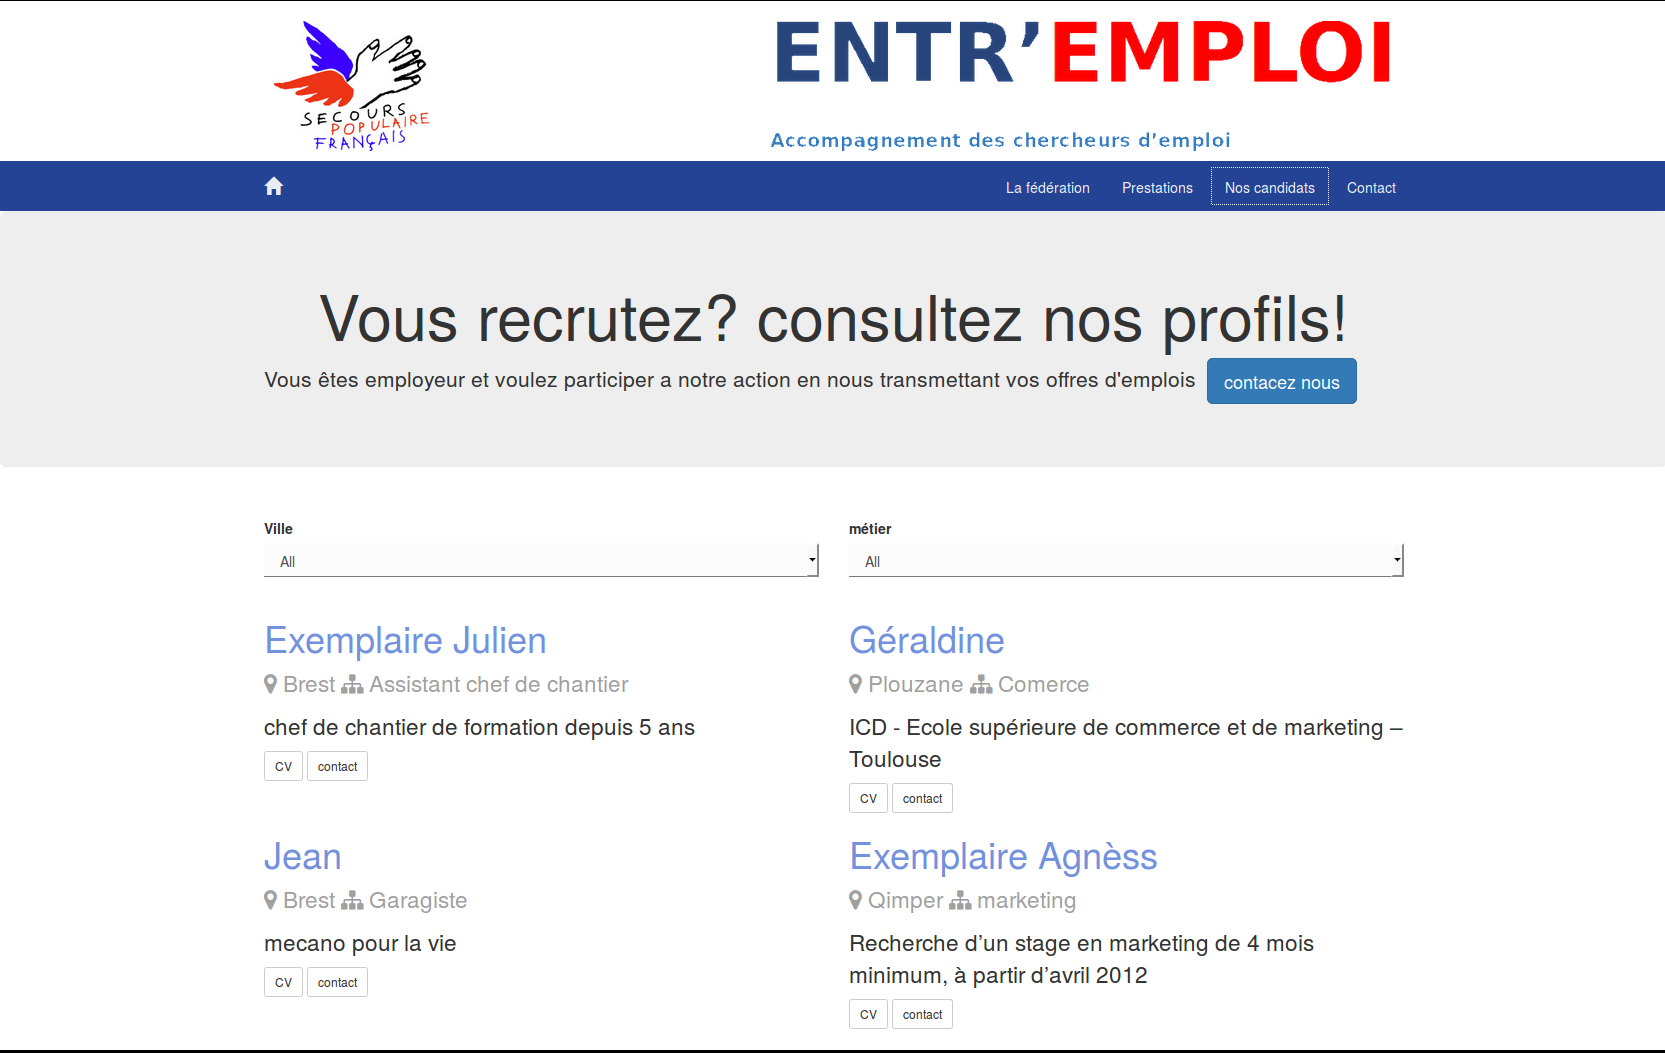
\includegraphics[width=16cm]{candidats.png}
\\
La page candidats affiche tous les CV mis en ligne par l'équipe Entr'Emploi. Pour visionner un CV l'entreprise doit entrer son adresse mail puis cliquer sur le lien qu'elle reçoit par mail.
\section{Contact}
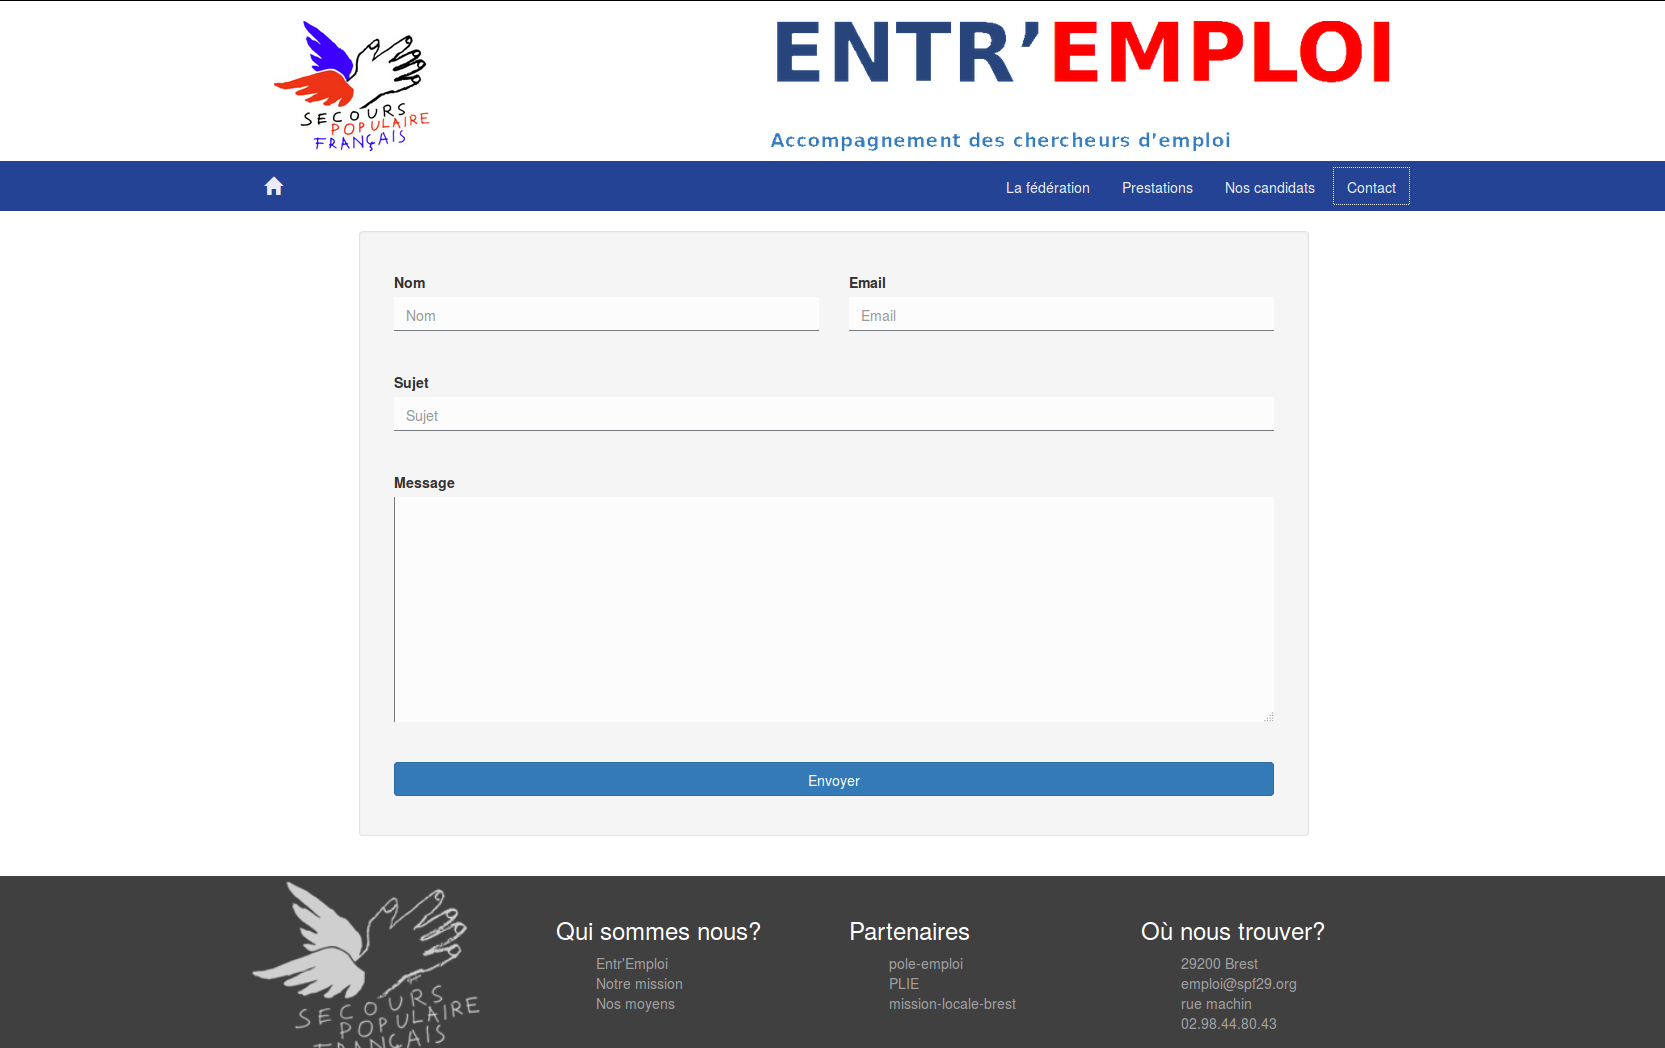
\includegraphics[width=16cm]{contact.png}
\\
La page de contact permet d'envoyer un mail a l'adresse emploi@spf29.org 

\chapter{Administration}
\section{Se connecter}
Pour vous connecter a la zone administrateur il faut que la personne en charge de la mise à jour du site vous crée un compte.
Une fois le compte créé rendez vous a l'adresse \url{http://entremploi-brest.org/admin} qui vous demandera vos identifiants et votre mot de passe.
\begin{center}
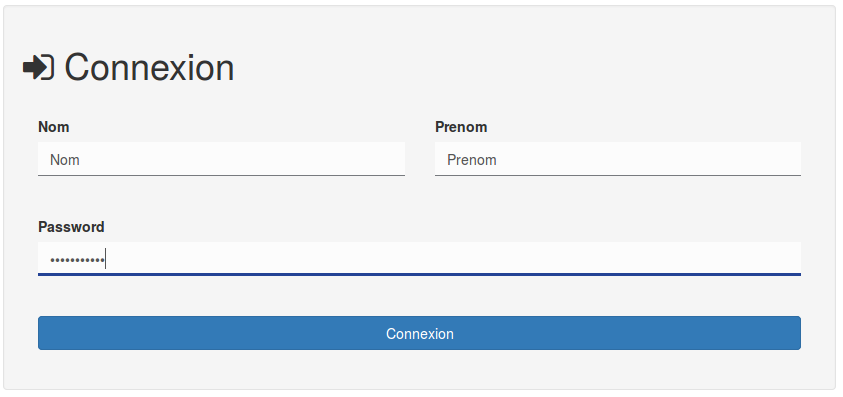
\includegraphics[height=5cm]{login.png}\\
\end{center}
Une fois vos identifiants entré cliquez sur connexion, un message apparaît alors:\\
\begin{center}
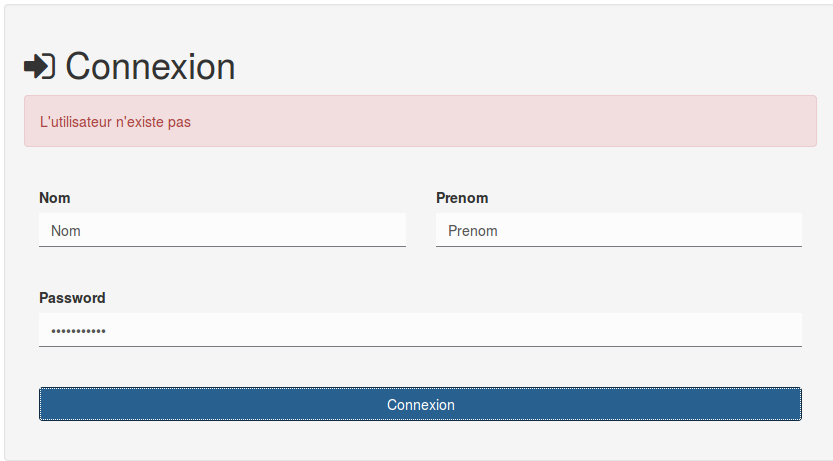
\includegraphics[height=5cm]{loginMessage.png}
\end{center}
Si le message indique "connexion valide", il suffit d'attendre quelques instants vous alez etre rediriger vers l'espace administrateur.\\
Si le message indique "l'utilisateur n'existe pas" Veuillez vérifier votre nom et prénom et vérifiez que votre compte a bien été créé par la personne en charge de la mise à jour du site.\\
Si le message indique "mauvais mot de passe" vérifier que vous avez bien entré votre mot de passe puis si cela ne fonctionne toujours pas demandez à la personne en charge de la mise à jour du site de changer votre mot de passe.

\section{Menu administrateur}
Si vous êtes bien connecté la page \url{http://entremploi-brest.org/admin} vous affiche ce menu:
\begin{center}
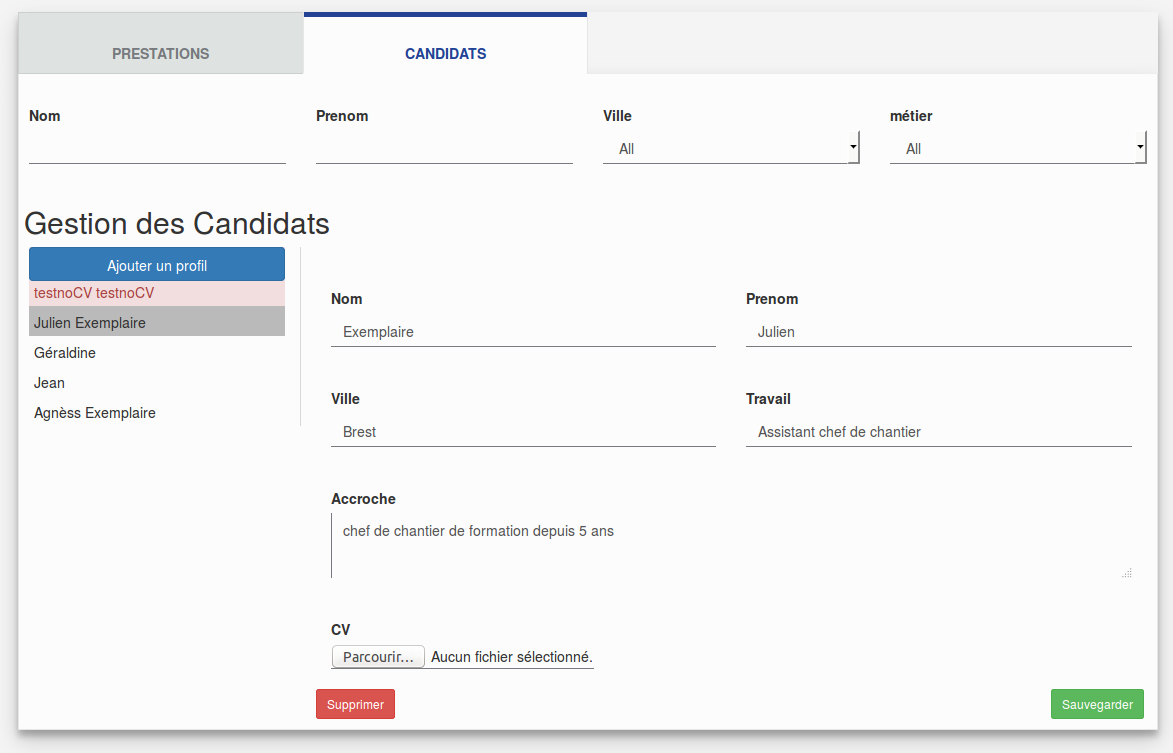
\includegraphics[width=16cm]{admin.png}
\end{center}
Pour passer d'une page a l'autre cliquez sur les onglets candidats ou prestations.

\section{Gestion des prestations}
\subsection{Ajout de prestation}
\subsection{Édition de prestation}
\subsection{Suppression de prestation}

\section{Gestion des candidats}
Le menu de gestion de candidat est le suivant:
\begin{center}
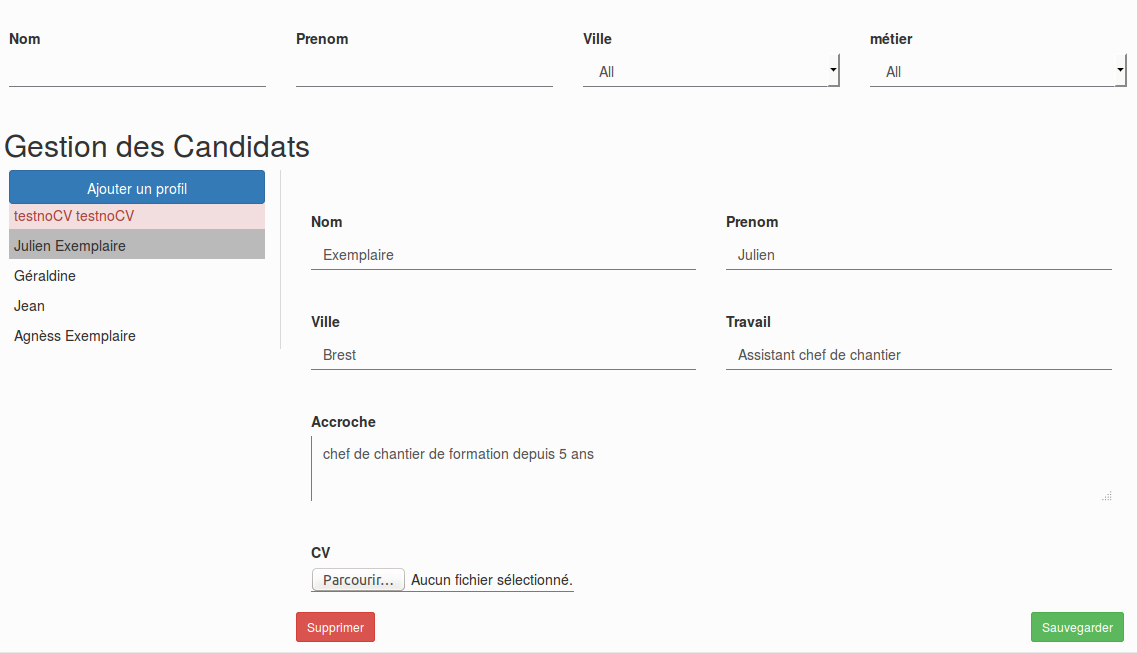
\includegraphics[width=16cm]{candidatsAdmin.png}
\end{center}
Il contient en haut un filtre de recherche pour chercher un candidat par son nom, prénom, ville ou métier.\\
A gauche vous trouverez la liste des candidats en fonction des valeurs entrée dans le filtre et pour finir à droite les information du candidat que vous pouvez modifier.\\
Les candidats sans CV sont en rouge.

\subsection{Ajout de candidat}
Pour ajouter un nouveau profil de candidat cliquez sur le bouton Ajouter profil en haut de la liste des profils. Ce formulaire apparait alors:
\begin{center}
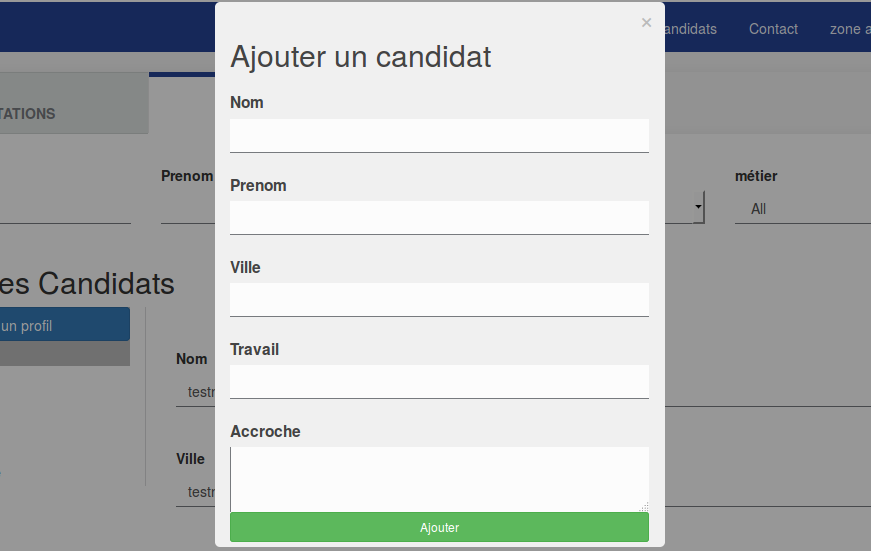
\includegraphics[width=16cm]{candidatsAdd.png}
\end{center}
Complétez les champs (le champ Nom est optionnel) puis cliquez sur le bouton vert Ajouter.
Le candidat est ajouté, vous pouvez le trouver dans la liste des candidats. Attention il n'a pas encore de CV.
\subsection{Ajout/Modification de CV}
Pour ajouter ou modifier un CV sélectionnez le candidat en question dans la liste des candidats a gauche puis cliquer sur parcourir:
\begin{center}
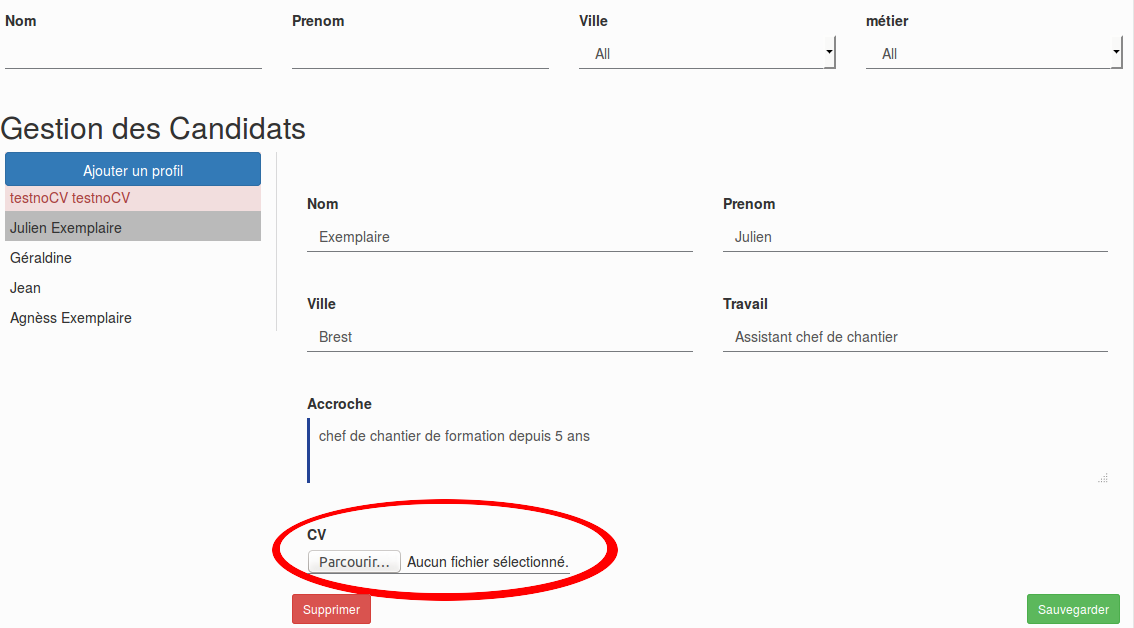
\includegraphics[width=16cm]{candidatsselectCV.png}
\end{center}
Une fois le CV en PDF choisis un bouton jaune Envoyer CV apparaît à coté du bouton vert Sauvegarder. Cliquez sur le bouton jaune et le CV est envoyé!
\begin{center}
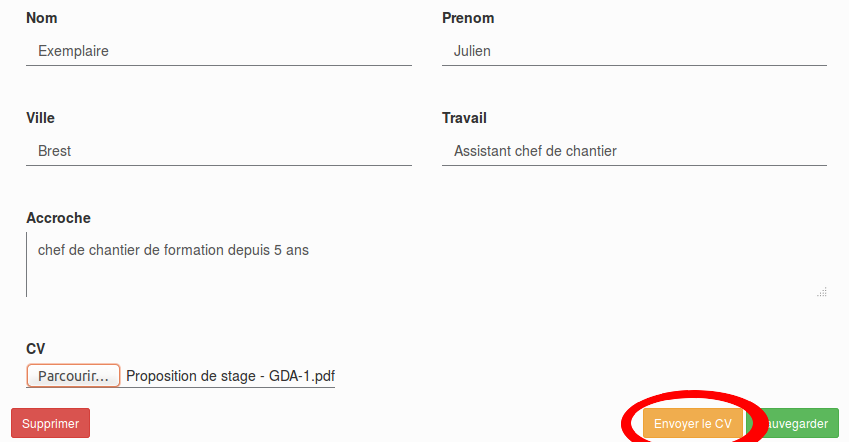
\includegraphics[width=16cm]{candidatssendCV.png}
\end{center}
\subsection{Édition de candidat}
Sélectionnez le candidat en question dans la liste des candidats a gauche, ses informations apparaissent alors à droite. Vous pouvez alors modifier les champs et cliquer sur le bouton vert Sauvegarder pour enregistrer les modifications.
\subsection{Suppression de candidat}
Sélectionnez le candidat en question dans la liste des candidats a gauche, Pour supprimer le candidat cliquez sur le bouton rouge "supprimer" en bas a gauche du formulaire.

\newpage
\section{Accès administrateur web}
L'Accès pour l'administrateur web est le même que pour tout le monde a l’exception qu'il a accès a deux onglets supplémentaires:
\begin{center}
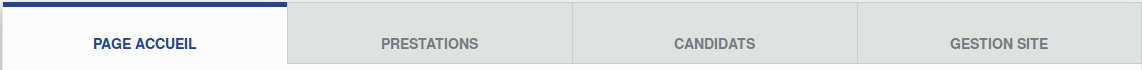
\includegraphics[width=16cm]{ongletsAdmin.png}
\end{center}
\subsection{Gestion page d'accueil}
\subsubsection{Carrousel}
Pour modifier les carrousel allez dans l'onglet Page Accueil, vous y trouverez une section édition du carrousel. Dans cette section vous pouvez ajouter une nouvelle image qui apparaîtra en première, supprimer ou modifier une image en cliquant sur les bouton "ajouter une image", "Supprimer" et "parcourir" puis modifier.
\begin{center}
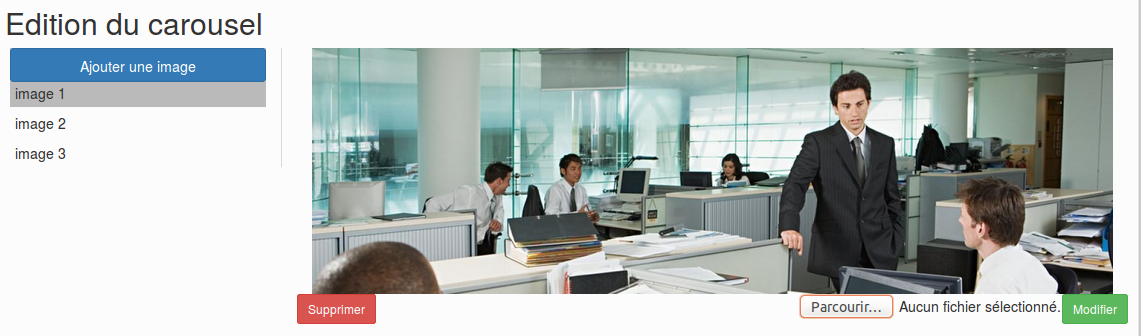
\includegraphics[width=16cm]{editionCarousel.png}
\end{center}
Attention lors de la sélection d'une image a ajouter ou modifier l'image peut mettre quelques secondes a apparaître surtout si elle est volumineuse.
\subsubsection{Articles page d’accueil}
\paragraph{Édition d'articles}
Après avoir sélectionné l'article que vous voulez éditer dans la liste de gauche vous pouvez modifier les champs comme vous le voulez puis cliquer sur modifier pour valider vos changements. Le champ position permet de donner un ordre d'apparition des articles sur la page d'accueil.\\
\paragraph{Joindre une image} à un article: Sélectionnez Image dans le menu déroulant média puis cliquez sur parcourir pour choisir l'image que vous voulez joindre. une fois l'image choisi sauvegarder les modifications
\begin{center}
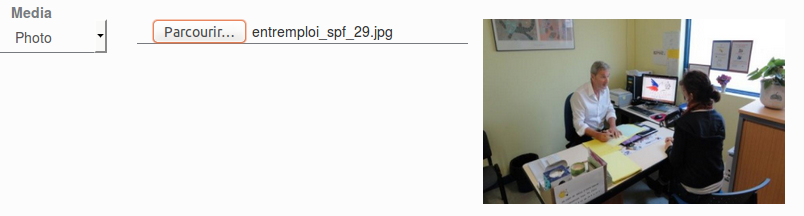
\includegraphics[width=16cm]{mediaImage.png}
\end{center}.
\paragraph{Joindre une vidéo} à un article, la vidéo doit être mise en ligne sur youtube. Copiez l'adresse de la vidéo du type: \url(https://www.youtube.com/watch?v=Cxd9lSINbVo) et collez la dans le champ "lien de la vidéo youtube" après avoir choisi vidéo dans le menu déroulant média. Sans oublier de sauvegarder les changements.
\begin{center}
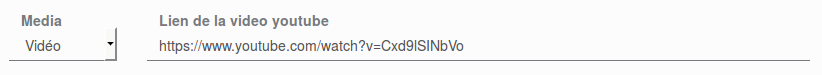
\includegraphics[width=16cm]{mediaVideo.png}
\end{center}
\paragraph{Ajout d'articles}
L'ajout d’articles se fait comme l'édition via le formulaire en bas de page dans la section "Ajouter un article".
\subsection{Gestion site}
\subsubsection{Changer les logos de haut de page}
Pour modifier un logo cliquez sur parcourir puis choisissez le logo que vous voulez. Attendez que le logo apparaisse puis si il vous convient cliquer sur le bouton "Valider".
\begin{center}
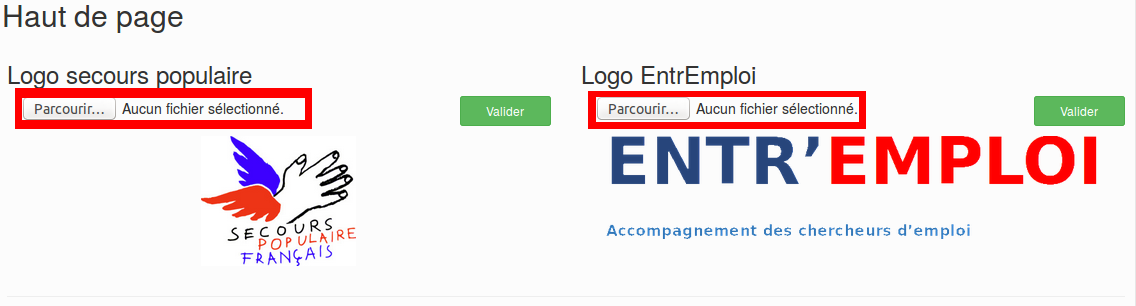
\includegraphics[width=16cm]{adminLogos.png}
\end{center}
\subsubsection{Gérer les comptes d’accès}
Les champs nom et prénom en haut permettent de rechercher un utilisateur par son nom et/ou son prénom.
La liste des utilisateurs apparaît a gauche et les informations sur l'utilisateur choisi sont à droite.\\
Pour ajouter a utilisateur cliquez sur le bouton "ajouter un utilisateur" au dessus de la liste des utilisateur et complétez le formulaire qui apparaît.
\begin{center}
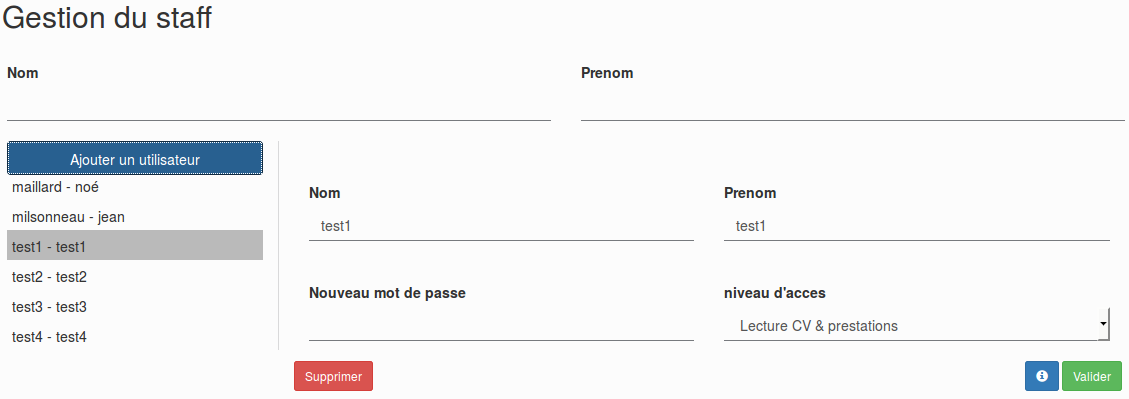
\includegraphics[width=16cm]{adminStaff.png}
\end{center}
\subsubsection{Gestion du pied de page}
\begin{center}
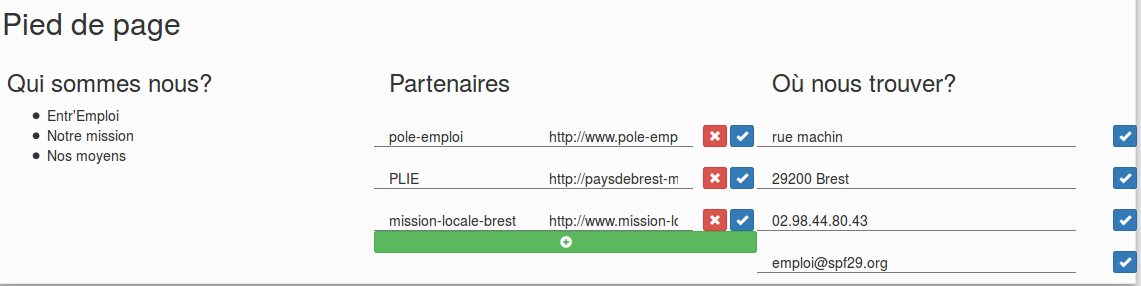
\includegraphics[width=16cm]{adminFooter.png}
\end{center}
\paragraph{Partenaires}
Vous pouvez modifier les partenaires existant et cliquer sur le bouton bleu pour valider les changement ou le bouton rouge pour supprimer le partenaire. Si vous voulez ajouter un partenaire cliquer sur le bouton vert et complétez le formulaire qui apparaît.
\paragraph{adresse}
Vous pouvez modifier les 4 champs d'adresse et cliquer sur le bouton bleu pour valider la ligne modifié.

\end{document}
